\subsection{Geometric proof (using Compactness)}

After the exhaustive proof of the previous section, we wanted to
refresh the reader with a totally different type of proof for SVD; one
that brings a new perspective for the way in which the special basis
for \R{n} is chosen. \\

Thinking about modular theorem proving, that is, factorizing common
results for the sake of clarity; one could consider that the 
\cref{thm:SVD1} and \cref{thm:SVD2} are some kind  of common step
for many possible SVD proofs. They deal with the task of proving that,
given certain condition over the bases in \R{n} and \R{m} ($A\vec{v_i}
= \sigma_i\vec{u_i}, \ds{\forall} i=1\dots\func{rank}(A)$); the SVD
factorization holds. Those auxiliary 
theorems then, reduce the task of proving the SVD 
\cref{thm:SVD} to the much more specific (but hard) subproblem of
finding the bases. Per discussion in previous section, we know
that such problem can be reduced even further, to the one of finding
the orthonormal basis for \R{n} $\{\vec{v_1},\vec{v_2},\dots,\vec{v_n}\}$, such
that its orthogonality is preserved through $A$
(\cite{kalman96}). This last remark can be considered the true essence of a
whole family of proofs for SVD Theorem, where each one brings a
particular way of finding a basis with such an special
property. \\

Intuitively, this property of preserving orthogonality could be
thought as a generalization of the eigenvectors behavior, which
are the vectors not ``moved'' by transformation $A$ but just scaled; this in
particular implies that if the eigenvectors formed an orthogonal basis
of the space prior application, their images under $A$ will still form a
basis (eigenvectors are defined when $A$ has signature $\R{n} \fromto
\R{n}$, which means $A$ is an square matrix). Something similar occurs
for the \vec{v}\apos{s} in SVD, but extended to a couple of spaces
instead of just one: we can not expect these vectors are not moved by
$A$, as they migrate of space ($\R{n} \fromto \R{m}$); but we request
that whatever landing they do on \R{m}, they still form an orthogonal
basis there. \\ 

The proof we are about to present now is thanks to Blank et al
\cite{blank89}; which presents a quite interesting approach: using
pure geometric arguments \footnote{With an implicit use of
  compactness} he finds the basis whose orthogonality under $A$ gets
preserved. \\

The whole reasoning occurs on the unit sphere and its image over an
square matrix $A$; and here comes a great connection with our previous
comments about the true essence of an arbitrary matrix $A$ of $m \times
n$ with rank $r$: the real information is on the mapping from the row
space to the column space ($\C{\trans{A}} \fromto \C{A}$), and
restricted to those subspaces $A$ is a bijection $\R{r} \fromto
\R{r}$; working with a 
bijective linear transformation means that $\inv{A}$ does
exist. Without loosing generality then, we will assume that matrix $A$ is
square and non-singular (invertible); because if it was not, we can do
a zoom and focus on its embedded bijection $\R{r} \fromto \R{r}$, and
calculate the basis there (and later extend to whole basis of host
spaces \R{n} and \R{m}). \\

The unit sphere is picked as the source of the \vec{v}\apos{s}, simply
because we want them to be an orthonormal basis (which in particular
requires them to be unitary). For starting to form this basis, we
could start picking an arbitrary unit vector; picking a second vector
in the sphere such that is perpendicular to the former is no issue
either; but how pick the second one such that the property the
property $\vec{v_1} \perp \vec{v_2}$ is preserved through $A$? Every
vector $\vec{v}$ in \R{r} defines a hyperplane $P$, 
which actually happens to be a subspace on its own. But such hyperplane
is actually the orthogonal complement of the subspace generated by
the vector alone; which implies that $P \perp \vec{v}$. So what? $P$
merely becomes an infinite source of orthogonal vectors to the second
choice \vec{v}; but the question of how to pick one such that the
orthogonality property gets preserved, is still unanswered. \\

The main point of the proof in \cite{blank89}, is that if we choose
properly the first vector \vec{v}, 
meaning if we choose the one which gets the maximum expansion through
$A$, then the orthogonality relation of \vec{v} with the hyperplane it
defines gets preserved. Here comes then a very powerful and beautiful
idea at the same time: having found a whole subspace that is
orthogonal to the first choice vector, allows one to forget about the
original host space \R{r} and focus on that subspace only; the new
hyperplane would essentially be \R{r-1} embedded in \R{r}, and the
intersection with the sphere in \R{r} would the unit sphere in
\R{r-1}. Thus, we can apply recursively the same procedure in that
subspace, for finding the next unit vector such that the
orthogonality of its hyperplane gets preserved through $A$! \\ 

Therefore, the theoretical recursive algorithm would be to find one vector
\vec{v_i} at a time, by working only on a subspace of dimension
$r-i+1$ (\vec{v_1} is found in whole \R{r}, \vec{v_2} is found in an
embedded \R{r-1}, \vec{v_3} in the nested embedded \R{r-2}, etc). If
we wanted to think in a proof rather than a constructive algorithm, we
could use induction and claim that we know how to find the first $r-1$
vectors \R{r-1}, and proceed to find the remaining vector in \R{r}. \\

We have reduced then, the problem of finding the right basis of
\vec{v}\apos{s} to the following theorem: \\

\begin{theorem}

\label{thm:svdgeo}
Let $A$ a non-singular matrix of $r \times r$; let be vectors
$\vec{v},\vec{w} \in \R{r} 
\suchthat A\vec{v} = \vec{w} \ds{\land} 
\norm{\vec{w}}_2 = \max\left\{\norm{\vec{x}}_2 \suchthat \norm{\inv{A}\vec{x}}_2= 1 \right\}$ 
and let $S$; $T$ be hyperplanes in
\R{r} $\suchthat$ $S$ is the orthogonal hyperplane of \vec{v}; and $T$
is image of $S$ under $A$ $\implies$ $T \perp \vec{w}$ ($T$ is also the
orthogonal hyperplane of \vec{w}).
\end{theorem}

To visualize the artifacts mentioned in the theorem, let us pay
attention then to the following picture, which is the unit 
sphere in $\R{r}$, mapped to an ellipsoid in $\R{r}$ \footnote{A
  formal argument is actually required to prove that the image of the
  unit sphere is an ellipsoid, and even telling that is the surface of
a quadratic form requires a little development. But we will omit those
details, aiming to keep the spirit of this short proof.} In order to
prove that $T \perp \vec{w}$, we will use the auxiliary hyperplanes
$S_1$ and $T_1$ (where the second is the image under $A$ of the
former). Of course the picture aims to represent \R{3}, and 
the hyperplanes would be embeddings of \R{2}; but let us just consider
them a visual representation of arbitrary dimension objects (the only
representation we can imagine, indeed). \\

\begin{figure}[h]
  \centering
  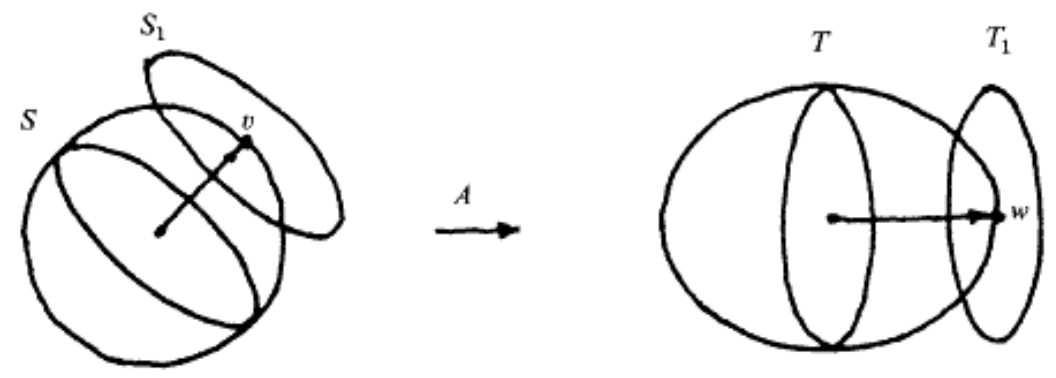
\includegraphics[width=13cm]{svd-geo-proof}
  \caption{Geometrical proof of SVD Theorem: Transformation $A$ preserves the
    relation $S \perp \vec{v}$}
  \label{fig:svdgeop}
\end{figure}
\hfill

\begin{proof}
The geometric proof goes like this: \\

\begin{enumerate}
\item The hyperplane $S_1$ touches the unit sphere only at point
  \vec{v}. It is a geometrical result that such hyperplane is unique
  and that $S_1 \perp \vec{v}$. \\

\item By definition, the hyperplane $T_1$ is the image of $S_1$ under
  $A$; also, the whole unit sphere is mapped by $A$ into an ellipsoid. Since
  $A$ is a bijective function, then $T_1$ must touch the ellipsoid only in
  point \vec{w} (just like $S_1$ touches the unit sphere only at point
  \vec{v}). Actually, $T_1$ must be the only hyperplane with such
  property (otherwise, we could apply \inv{A} to that other hyperplane,
  and it would produce a different hyperplane that also touches
  \vec{v} in the unit sphere; contradicting previous point about the
  uniqueness of $S_1$). \\

\item Now take another sphere, big enough to cover the deformed image of
  the unit sphere under $A$ (the ellipsoid). Start to shrink
  such sphere until it touches the ellipsoid for the first time; per
  definition, \vec{w} must be part of those points of first
  contact. \\

\item Now consider the hyperplane $T_2$ that touches this shrunk sphere,
  precisely at \vec{w}. Using the same geometrical theorem of first
  argument about $S_1$, we can tell such hyperplane is unique and is
  orthogonal to \vec{w}. \\

\item Since this adjusted sphere covers entirely the ellipsoid (per
  definition of \vec{w}), then $T_2$ also touches the ellipsoid at
  point \vec{w}. But we argued that $T_1$ was the only hyperplane
  touching the ellipsoid at \vec{w} $\implies$ $T_1 = T_2 \ds{\land} T_1
  \perp \vec{w}$. \\

\item Both hyperplanes $S$ and $S_1$ are orthogonal to \vec{v}; by
  geometrical arguments they must be parallel then. \\

\item Linear transformations, in particular $A$, preserve parallelism;
  since, $S \parallel S_1$ $\implies$ their respective images under $A$
  must be parallel as well. \\

\item The image of $S_1$ under $A$ is $T_1$, then, whatever becomes
  the image of $S$ under $A$; it must be parallel to $T_1$. Let us
  call this image $T$. \\

\item $\therefore$ $T \parallel T_1 \ds{\land} T_1 \perp \vec{w}$
  $\implies$ $T \perp \vec{w}$.  
\end{enumerate}
\end{proof}
\hfill

The key choice in the proof was \vec{w}, as being the biggest axis of
the ellipsoid makes it coincide with the sphere of radius
$\norm{w}_2$; and that in turns allows us to transfer the properties
of the hyperplane that touches the sphere at \vec{w} to the one that
touches the ellipsoid at same point (as they become same hyperplane
indeed). It is no coincidence then, that the spectral norm $\norm{A}_2$
is actually defined as $\norm{\vec{w}}_2$; that is, is defined
as the maximum expansion $\norm{A\vec{x}}_2$ that transformation $A$ causes
on the vectors belonging to the unit sphere. This norm actually, is
used in the algebraic proof of Golub in \cite{golub13}, of the SVD
Theorem. \\ 

The last question the reader may have now is: where was the
compactness property used? It may not be explicitly stated, but it
lies behind the definition of \vec{w}: $\norm{\vec{w}}_2 =
\max\left\{\norm{\vec{x}}_2 \suchthat \norm{\inv{A}\vec{x}}_2 = 1
\right\}$. The reason why \vec{w} exists 
on the first place, is because the ellipsoid is a compact set (it
inherits that property from its pre-image, the unit sphere, thanks to
the continuity of function $A$\footnote{Though we did not find the
  name for such theorem, it must exists and state that continuous
  functions preserve compactness.}). Since the norm function $\norm{.}_2$
is also continuous, then by a generalization of the Extreme Value
Theorem from Calculus, it must reach its maximum on a point of the
ellipsoid (we named that particular point as \vec{w} in the proof). \\

